\begin{exsol}{19}{Cabral 7.14 Centipede}{182}{Exam}{B2}
\asked For the centipede game of Cabral's Figure~7.13, show by backward induction that rational
players stop ($d$) at every node, giving payoffs $(2,0)$, then judge whether this equilibrium is
reasonable and state the rationality assumptions behind it.

\method Backward induction and subgame perfection (Cabral \S7.2, pp.~167--169); the same
unravelling as the finitely repeated game (Exercise 7.13, \S7.3). The game is due to Rosenthal
(1981) (Cabral, ch.~7 note~6). Course link: backward induction in alternating offers (notes,
Aula~2) and reputation as a substitute for contracts (\MR{} pp.~139--140).

\solution
\subparagraph{(a) The game.} Reading Figure~7.13 (p.~182): players alternate, Player~1 at the odd
nodes and Player~2 at the even nodes; at each node the mover either stops ($d$) or continues
($r$). The stopping payoffs (Player~1, Player~2) are
\[
\text{node } 2j-1 \text{ (P1)}:\ (2j,\ 2j-2), \qquad
\text{node } 2j \text{ (P2)}:\ (2j-1,\ 2j+1), \qquad j = 1,\dots,50,
\]
which reproduces every vector printed in the figure: $(2,0)$, $(1,3)$, $(4,2)$, $(3,5)$,
$(6,4)$ at the start and $(97,99)$, $(100,98)$, $(99,101)$ at the end, with $(100,100)$ if
Player~2 continues at the last node. The pattern implies 100 decision nodes; the argument below
does not depend on the length.
\begin{center}
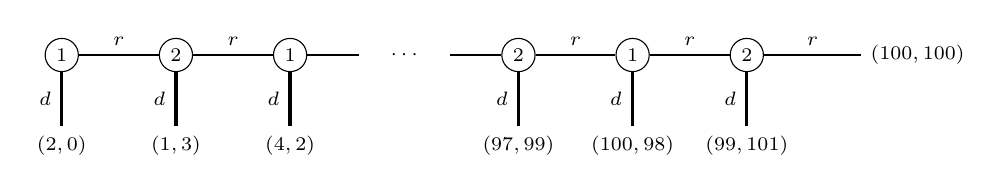
\begin{tikzpicture}[x=1.45cm, every node/.style={font=\scriptsize},
  dec/.style={circle,draw,inner sep=1.2pt,minimum size=12pt}]
  \foreach \i/\p/\pay in {1/1/{(2,0)},2/2/{(1,3)},3/1/{(4,2)},5/2/{(97,99)},6/1/{(100,98)},7/2/{(99,101)}}{
    \node[dec] (n\i) at (\i,0) {\p};
    \draw[very thick] (n\i) -- node[left] {$d$} (\i,-0.9);
    \node at (\i,-1.15) {$\pay$};
  }
  \draw (n1) -- node[above] {$r$} (n2);
  \draw (n2) -- node[above] {$r$} (n3);
  \draw (n3) -- (3.6,0); \node at (4,0) {$\cdots$}; \draw (4.4,0) -- (n5);
  \draw (n5) -- node[above] {$r$} (n6);
  \draw (n6) -- node[above] {$r$} (n7);
  \draw (n7) -- node[above] {$r$} (8,0) node[right] {$(100,100)$};
\end{tikzpicture}
\end{center}

\subparagraph{(b) Backward induction.} Start at the last node and move left; at each node the
mover compares stopping with the continuation value found one step earlier.
\begin{center}\small
\begin{tabular}{@{}cccccc@{}}
\toprule
Node & Mover & Payoff to mover if $d$ & Payoff to mover if $r$ & Choice & Value carried left \\
\midrule
100 & P2 & 101 & 100 (end) & $d$ & $(99,101)$ \\
99 & P1 & 100 & 99 (P2 stops at 100) & $d$ & $(100,98)$ \\
98 & P2 & 99 & 98 (P1 stops at 99) & $d$ & $(97,99)$ \\
$\vdots$ & & & & $\vdots$ & \\
$2j$ & P2 & $2j+1$ & $2j$ & $d$ & $(2j-1,2j+1)$ \\
$2j-1$ & P1 & $2j$ & $2j-1$ & $d$ & $(2j,2j-2)$ \\
$\vdots$ & & & & $\vdots$ & \\
2 & P2 & 3 & 2 & $d$ & $(1,3)$ \\
1 & P1 & 2 & 1 & $d$ & $(2,0)$ \\
\bottomrule
\end{tabular}
\end{center}
The general step: at a P1 node $2j-1$, continuing leads (by the step already solved) to P2
stopping at $2j$, which gives P1 $2j-1 < 2j$; at a P2 node $2j$, continuing leads to P1 stopping
at $2j+1$, which gives P2 $2j < 2j+1$. At every node the mover gains exactly one unit by stopping
before the other does. Hence $d$ at every node is the unique subgame-perfect equilibrium
(preferences are strict), and the game ends at once with $(2,0)$.

\subparagraph{(c) Is it reasonable?} Normatively it is compelling step by step, yet the outcome
is very poor: total payoff $2$ against $200$ if both always continued, and \emph{both} players
would get at least $97$ by reaching the last nodes. Three objections:
\begin{enumerate}[label=(\roman*)]
  \item \emph{Evidence.} In laboratory versions of the game, few subjects stop at the first node;
  most play continues for several rounds before someone stops (McKelvey and Palfrey, 1992,
  \emph{Econometrica} 60(4)). Cabral's Exercise 7.16 invites exactly this kind of test.
  \item \emph{Off-path reasoning.} The argument asks Player~2 at node~2 to assume Player~1 will
  stop at node~3, although reaching node~2 is evidence that Player~1 does \emph{not} play as the
  theory says. Once one deviation has been observed, it is not obvious why the rest of the
  theory should be believed.
  \item \emph{A small doubt is enough.} If Player~2 assigns even a small probability to Player~1
  being a ``cooperator'' who continues, a rational Player~1 gains by imitating that type for a
  while, and continuation for many rounds becomes equilibrium behaviour (the reputation logic of
  Kreps, Milgrom, Roberts and Wilson, 1982; \MR{} pp.~139--140).
\end{enumerate}

\subparagraph{(d) The rationality assumptions.} The prediction needs (1) each player is rational
(maximizes own payoff, with no altruism or fairness concerns, cf.\ \MR{} FFT~5.1, item~20);
(2) payoffs and the game are common knowledge; and (3) \emph{common knowledge of rationality} to
depth about 100: P1 must know that P2 knows that P1 knows \dots that the last mover is rational,
and must expect this belief to survive after deviations. Assumption (3) is the demanding one,
and it is the one the experiments and the reputation argument relax.

\interp The centipede is a model of trust in a relationship with a known end. Each period both
gain by continuing, but each is tempted to grab the slightly larger share now; backward
induction from the known last date unravels cooperation completely, as in the finitely repeated
prisoner's dilemma (Exercise 7.13). For organizations the lesson is that long relationships
sustain cooperation through reputation and uncertainty about the other side's type, not through
the logic of a fixed, commonly known horizon; and the same backward-induction tool that fails
here as a prediction is the right tool for alternating-offers bargaining with few rounds.

\verify (1) The script \texttt{check\_B.py} runs backward induction over all 100 nodes, recovers
$d$ everywhere and $(2,0)$, and checks that every stopping vector printed in the figure matches
the formula. (2) Stronger result: every Nash equilibrium (not only the subgame-perfect one)
ends at node~1. Suppose an equilibrium path reached some node $k>1$ and ended there with a stop
by the mover at $k$ (or at the terminal vector after node 100). The mover at $k-1$ would then
get one unit less than by stopping at $k-1$ (the computation in (b)), and at the terminal vector
P2 would gain $1$ by stopping at node 100; so the profile is not a Nash equilibrium. Only paths
that stop at node~1 survive.

\answer{Backward induction: at node $2j$ Player~2 gets $2j+1$ by stopping and $2j$ by
continuing; at node $2j-1$ Player~1 gets $2j$ against $2j-1$. So $d$ is chosen at every node and
the unique SPE gives $(2,0)$, against up to $(100,100)$. Every Nash equilibrium has the same
outcome. The prediction relies on rational, self-interested players and common knowledge of
rationality to depth about 100. It is unreasonable as a forecast: experiments show prolonged
continuation, and a small doubt about the other's type rationalizes it.}
\end{exsol}
